\subsection{Meshes, Point-Clouds and Voxels}\label{MPCV}

\textbf{Meshes}~--~A mesh is a geometric data structure used to represent the surfaces of 3D objects through subdivisions into a network of polygons. These polygons are typically formed by vertices connected by edges, creating faces or facets. Meshes are pivotal in computer graphics and 3D modeling for their ability to represent complex surfaces efficiently, facilitating accurate rendering and transformation \citep{lahav2020meshwalker, Zhang_2023}.

\textbf{Point-Clouds}~--~A point cloud is a collection of data points in a 3D coordinate system (X, Y, Z). They offer quick rendering and transformation capabilities, which is advantageous for direct inspection. However, point clouds may not integrate seamlessly into sophisticated 3D applications that primarily use mesh-based rendering \citep{voxels, Zhang_2023}.

\textbf{Voxels}~--~A voxel is analogous to a 3D pixel, representing the smallest unit in a voxel-based model~-~a collection of 3D pixels. It is a discretized model primarily associated with solid modeling. In point cloud data, voxels can be used to represent each point, providing a filled view of the spaces between points \citep{voxels, Zhang_2023}.

\begin{figure}[H]
    \centering
      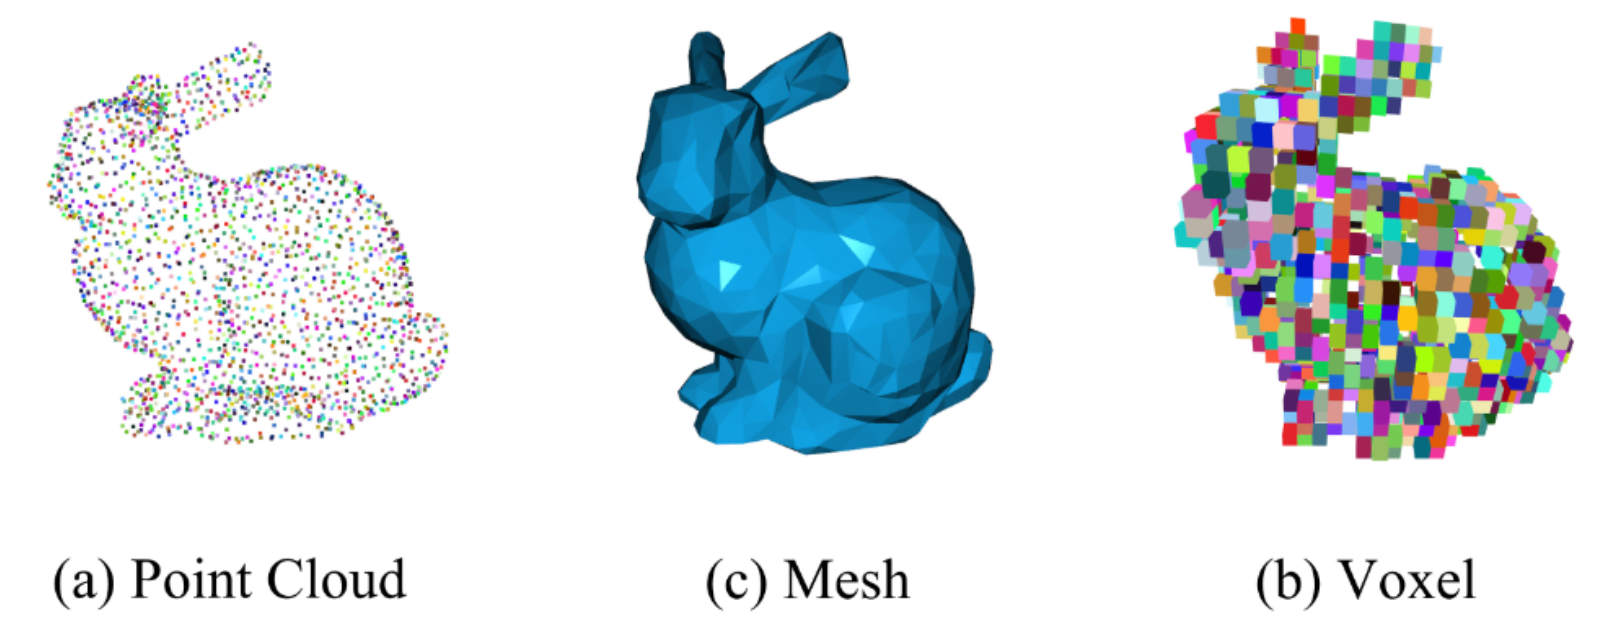
\includegraphics[width=.8\columnwidth]{figures/basics/mpcv.png}
      \caption{Representation forms of 3D data, adapted from Zhang et al.~\citep{Zhang_2023}.}~\label{fig:mpcv}
\end{figure}